\documentclass{IEEEtran}
\usepackage[utf8]{inputenc}
\usepackage[load=named]{siunitx}
\usepackage{amsmath}
\usepackage{graphicx}
\usepackage{tabularx}

\graphicspath{{images/}}



\begin{document}

\title{Recurrent Networks}
\author{
	\IEEEauthorblockN{J.R. Powers-Luhn}
	\IEEEauthorblockA{
    	Department of Nuclear Engineering\\
		University of Tennessee\\
		1004 Estabrook Rd\\
		Knoxville, TN 37996\\
		Email: jpowersl@vols.utk.edu
    }
}
\date{July 5th, 2017}

\maketitle

\section{Objectives\label{sn:objectives}}
The objective of this research is to examine the relative merits of recursive neural network architectures.

\section{Methodology\label{sn:methodology}}
Training data were created by taking the sine of numbers in the range [0.0, 0.5, 1.0, ..., 61.5, 62.0] for a total of 125 points. To this was added random noise in the range of [0, 1]. The variance of this data was measured to be 0.003, which was used as the mean squared error training goal of all networks trained in this experiment. Each network was trained based on the first sixty points in the input data set in an effort to determine whether or not it could predict ahead reliably. Each of the networks described below was trained for a maximum of 1000 epochs.

A multilayer feed forward network with four hidden neurons was trained as a benchmark. The network was trained to predict the sinusoid two steps ahead, e.g. $ \sin{x_i} \rightarrow \sin{x_{i+2}} $.

The first time-aware network tested was a time-delay neural network. It was trained with one delayed input, attempting to fit $ f\left(\sin{x_i}, sin{x_{i-1}}\right) \rightarrow \sin{x_{i+1}} $. Several networks were generated in an effort to find the minimum number of hidden neurons that trained the network to within the error goal by or before 1000 epochs.

Next, a Jordan network was generated using the \verb|narxnet| command in Matlab. No delayed inputs were employed. The number of recurrent, or feedback, delays was adjusted in order to determine the minimum viable number, as was the number of neurons in the hidden layer.

Finally, an Elman network was trained, again with no delayed inputs. The Matlab \verb|elmannet| command was used to create several networks, again with the goal of minimizing the number of neurons in the hidden layer while still meeting performance goals.

\section{Results\label{sn:results}}
\subsection{Feed forward network\label{sn:feedforward}}
Efforts to train the feed forward network were unsuccessful. A fit of the training data is shown in figure \ref{fig:ffnetperf}. As shown in figure \ref{fig:feedforward_performance}, the best this network could accomplish was a crude remapping of the input data. This was as expected, as the input-output mapping is fundamentally degenerate--the same input could correspond to multiple outputs, depending on whether the slope of the sinusoid function is positive or negative in that region.

\begin{figure}[ht]
    \centering
    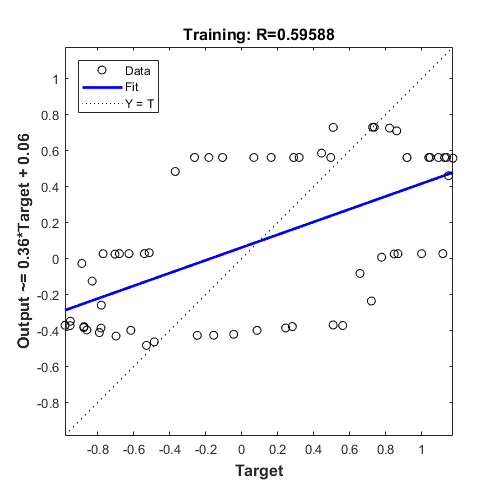
\includegraphics[width=\linewidth]{feedforward/feedforward_regression}
    \caption{Performance of feed forward network with four hidden neurons \label{fig:ffnetperf}}
\end{figure}

\begin{figure}[ht]
    \centering
    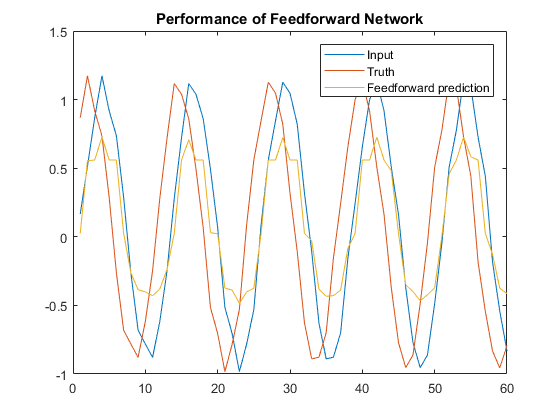
\includegraphics[width=\linewidth]{feedforward/feedforward_performance}
    \caption{The feed forward network did not accurately model the sinusoid function \label{fig:feedforward_performance}}
\end{figure}

\subsection{Time-delay network\label{sn:tdnn}}
Since the function being modeled fundamentally depended on both the input value and the derivative, it was expected that a time delay network would be more successful. The network was trained with a single delayed input with the architecture shown in figure \ref{fig:tdarch}.

It was determined that the minimum number of neurons required to train to the specified error within 1000 epochs was 36. A network this large appreciably increased the amount of time required to train. However, increasing the delay to include the two points previous to the one being predicted enabled a network (shown in figure \ref{fig:bettertd}) to reach the training goal with only 7 neurons. Even this network, however, did not fit the full data set within error (figure \ref{fig:tdperf}), with a final mean squared error on the combined training and evaluation data of 0.0091. This network type is limited based on the number of delayed-inputs provided. Each additional delayed input allows one order of higher approximation, essentially following the Taylor series expansion of the original function. Since this network only has one or two delayed inputs, the higher order derivatives are not available and the function approximation suffers.

\begin{figure}[ht]
    \centering
    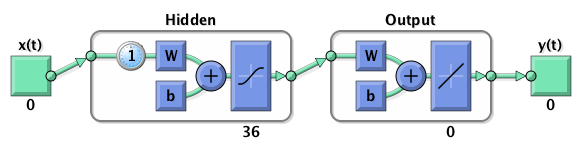
\includegraphics[width=\linewidth]{timedelay/diagram}
    \caption{Notional diagram of the successfully trained time delay network \label{fig:tdarch}}
\end{figure}

\begin{figure}[ht]
    \centering
    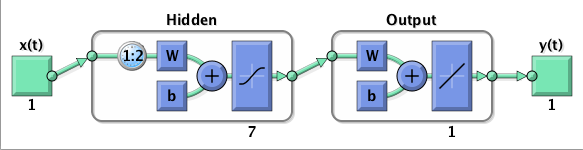
\includegraphics[width=\linewidth]{timedelay/better_tdnn}
    \caption{Smaller network employing two delayed inputs \label{fig:bettertd}}
\end{figure}

\begin{figure}[ht]
    \centering
    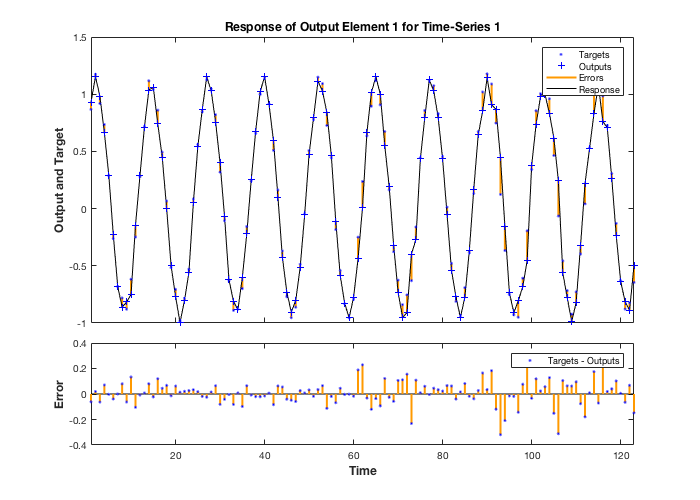
\includegraphics[width=\linewidth]{timedelay/tdnn_more_feedback_perf}
    \caption{Performance of two-feedback network on evaluation set \label{fig:tdperf}}
\end{figure}

\subsection{Jordan network \label{sn:jordan}}
The Jordan network was significantly more successful. A small network with only one hidden neuron (see figure \ref{fig:narxnet}) was able to predict the one-step-ahead, even when reading only its own output and a single input. The performance of this network was well within the error standard, even when predicting the full 120+ points in the original data set, as shown in figure \ref{fig:narxperf}.

\begin{figure}[ht]
    \centering
    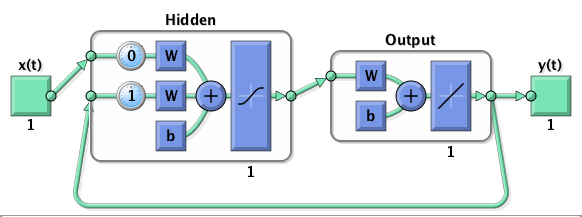
\includegraphics[width=\linewidth]{narx/closed_loop}
    \caption{Jordan network (closed) \label{fig:narxnet}}
\end{figure}

\begin{figure}[ht]
    \centering
    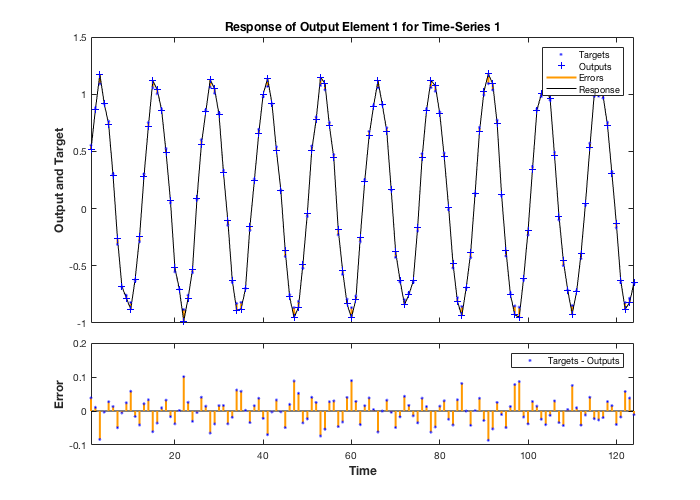
\includegraphics[width=\linewidth]{narx/closed_loop_full}
    \caption{Jordan network (closed) \label{fig:narxperf}}
\end{figure}

Unlike the time-delayed network, the Jordan network is fully recursive. This architecture allows the network to maintain its state in memory, allowing for more complex relationships.

\subsection{Elman network \label{sn:elman}}
The Elman network (figure \ref{fig:elman}) trained for this experiment performed similarly to the Jordan network in section \ref{sn:jordan}. Indeed, this was effectively the same network, except for the removal of the linear layer from the feedback signal. Performance for the entire data set is shown in figure \ref{fig:elmanperf}. 

\begin{figure}[ht]
    \centering
    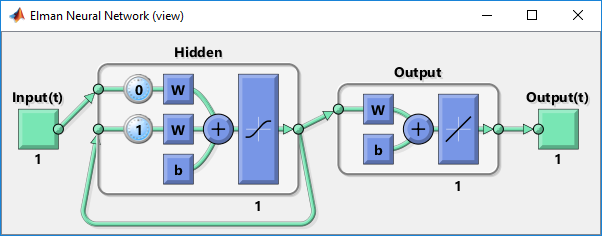
\includegraphics[width=\linewidth]{elman/net}
    \caption{Elman network architecture \label{fig:elman}}
\end{figure}

\begin{figure}[ht]
    \centering
    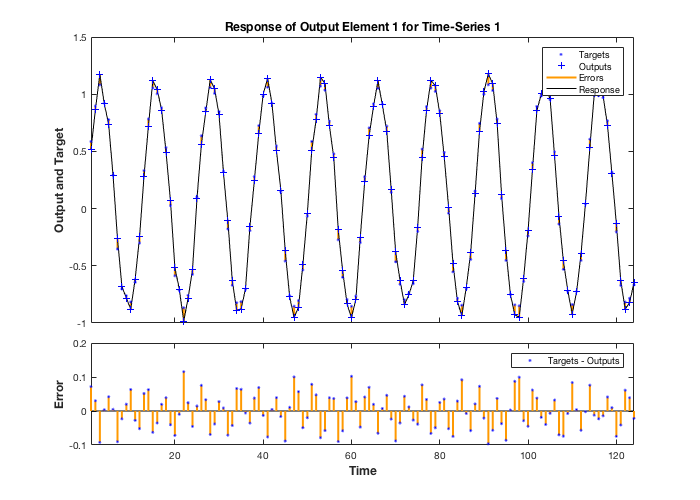
\includegraphics[width=\linewidth]{elman/full_data_perf}
    \caption{Elman network performance \label{fig:elmanperf}}
\end{figure}

While the Elman network resembles the Jordan network, the stored state does not represent values in the input or output set. Instead, it represents some intermediate value in the network. It is possible that this would provide benefit to more complex calculations by allowing for a greater degree of non-linearity. For this application, however, the performance is similar to that of the Jordan network.

\section{Conclusions}
An examination was made comparing the performance of various recurrent networks at predicting time series data. A feed forward network, which must make a prediction based only on current data, was shown to be a poor model for predictions of future values of time series data. A time delay network performed better, but still required several neurons to account for higher order functions (since it does not maintain a state vector). Jordan and Elman networks, by contrast, do maintain this state in some form, allowing them to make accurate predictions recursively, even dozens of time steps in the future. The output of the networks examined in this paper only depended on their own earlier values; it would be interesting to examine their performance in predicting values that had a periodic component in addition to trend lines that depended on other values (rather than random noise). Training these networks might require more complex architecture decisions in order to achieve required accuracy.

\end{document}
